\documentclass[a4paper,11pt]{article}
\usepackage[utf8]{inputenc} % Required for inputting international characters
\usepackage[T1]{fontenc} % Output font encoding for international characters
\usepackage[italian]{babel} % Italian dictionary
\usepackage{siunitx} % SI
\usepackage{amsmath}

\usepackage{graphicx} % cooler tables
\usepackage{wrapfig} % tables/images alignment

\usepackage{bm}
\usepackage{tikz}
\usepackage{hhline}
\usepackage{listings}

\usepackage[margin=2cm, includefoot]{geometry} % Modify margins
\usepackage{fancyhdr}
\usepackage{rotating}
\usepackage[hidelinks]{hyperref} % Hyperlinks

\usepackage[none]{hyphenat}% Non spezza le parole nelle tabelle
\usepackage{array}

\usepackage{graphicx} % Required for figures
\usepackage{float}
\usepackage{caption}
\usepackage{subcaption}

%pagestyle
\pagestyle{fancy}
\fancyhead{}
\fancyfoot{}
\fancyfoot[R]{\thepage}
\renewcommand{\headrulewidth}{0pt}


\usepackage{xfrac}
\usepackage{amssymb}

\usepackage{multicol}
\usepackage{multirow}

\usepackage[toc, page]{appendix}
\usepackage{booktabs}

\begin{document}
% TODO: distringuere Vin e VG
% TODO Dire che Vin < Vg
\section{Obiettivi}
\begin{enumerate}
	\item Verifica della linearità degli amplificatori operazionali e misura del guadagno di un circuito amplificatore.
	\item Misura della frequenza di taglio di un filtro passa alto e verifica del suo comportamento derivatore.
	\item Verifica dell'effetto di somma di un circuito sommatore invertente.
\end{enumerate}

\section{Apparato Sperimentale}
Gli strumenti che si utilizzano nel corso dell'esperienza sono i seguenti:
\begin{itemize}
	\item Multimetro digitale Tenma 72-13430
  	\item Oscilloscopio-generatore di funzioni Picoscope 2204A con due sonde di compensazione
	\item Circuito integrato TL082 contenente due amplificatori operazionali
	\item Breadboard con scheda di alimenatazione $0/5\,\si{\volt}$, $-12/0/12\, \si{\volt}$
	\item Alimentatore di tensione continua $5\,\si{\volt}/1.6\,\si\ampere$
	\item Tre resistori $R_1$, $R_f$, $R_3$ e tre condensatori $C_1$, $C_{a+}$, $C_{a-}$
\end{itemize}

\section{Amplificatore Operazionale Invertente}
Lo scopo di questa sezione è quello di studiare il comportamento di un circuito resistivo comprendente un amplificatore operazionale in configurazione invertente. In particolare, ci si propone di verificarne il comportamento lineare e di misurarne l'amplificazione, sia da una misura delle resistenze $R_1$ e $R_f$, sia dall'interpolazione lineare di misure acquisite con l'oscilloscopio.

\subsection{Configurazione Sperimentale}

Innanzitutto è necessario preparare l'alimentazione dell'operazionale, collegando le uscite
$+12\,\si{\volt}$ e $-12\,\si{\volt}$ ai pin n.8 e n.4 dell'operazionale.
Inoltre, a causa dell'alto guadagno, sono state collegate due capacità
$C_{a-}\approx C_{a+} \approx 100\si{nF}$ tra la massa e l'alimentazione invertente e non invertente
rispettivamente, con l'obiettivo di minimizzare i fenomeni di oscillazione.

%------------------------------------
\begin{wrapfigure}{r}{0.5\textwidth}
\centering
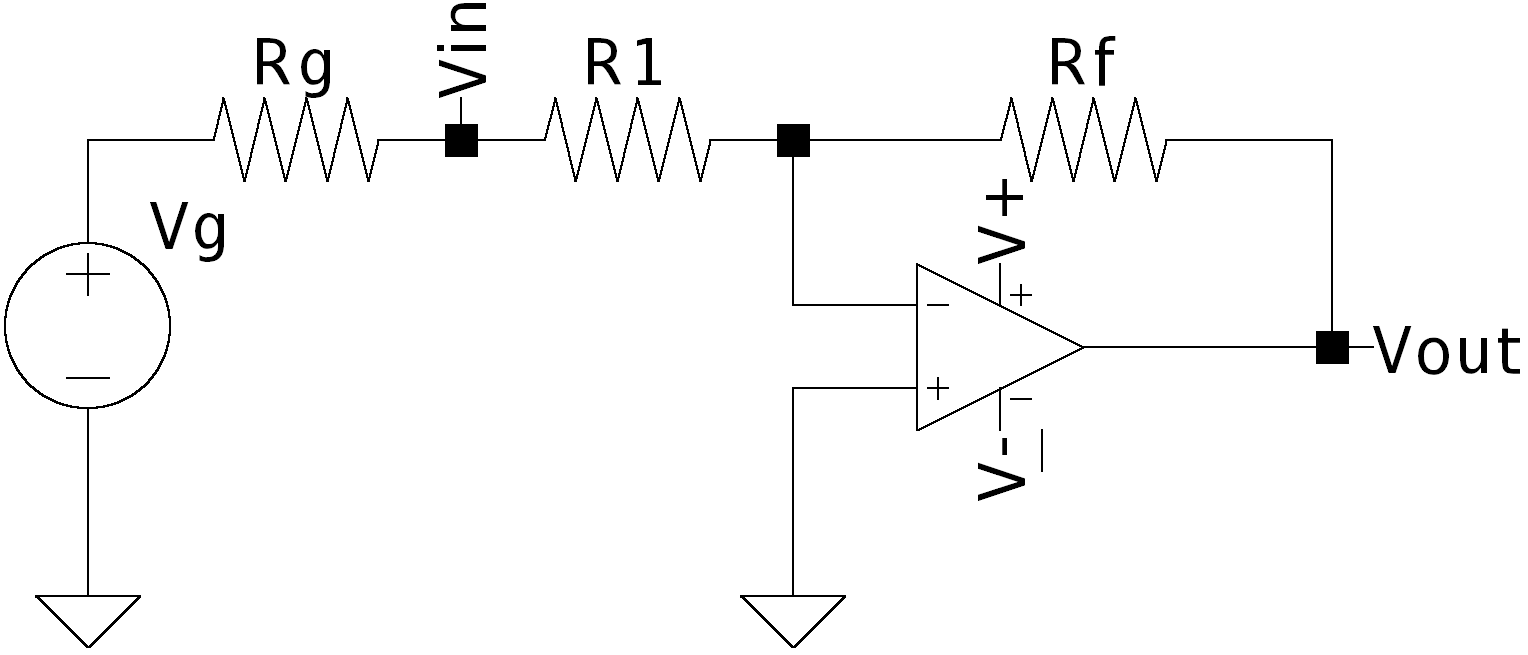
\includegraphics[width=0.5\textwidth]{images/circuit_inv}
\caption{\footnotesize Rappresentazione a costanti concentrate del circuito utilizzato.
  Si mettono in evidenza, oltre alle resistenze $R_{1}$ e $R_{f}$, la resistenza del
generatore $R_{G}$.}
\label{fig:wrapfig}
\end{wrapfigure}
%------------------------------------
Successivamente è stato assemblato sulla breadboard il circuito rappresentato in Figura \ref{fig:wrapfig}
ed è stato prelevato il segnale nei punti $V_{in}$ e $V_{out}$ utilizzando le sonde
$10X$ collegate ai canali A e B dell'oscilloscopio. I valori delle resistenze utilizzati sono stati
misurati direttamente con il multimetro e sono riportati nella Tabella \ref{tab:resist}.
Inoltre, il Picoscope è stato configurato in modo da compensare l'attenuazione del segnale dovuta dalla sonda e in modo da far erogare al generatore di funzioni incorporato un segnale sinusoidale di $1\,\si{kHz}$, con ampiezza picco-picco inizialmente di $0.2\, \si{\volt}$, aumentata gradualmente fino a $4\,\si{\volt}$.


Risolvendo il circuito e assumendo ideale l'amplificatore operazionale ci si aspetta che
il segnale in ingresso venga amplificato di un fattore $G = \frac{R_{f}}{R_{1}}$.
Inoltre, il segnale di output sarà invertito rispetto a quello di ingresso, in modo
da soddisfare la relazione $V_{out}=-G\, V_{in}$. Facendo riferimento ai valori riportati
in tabella \autoref{tab:resist} ci aspetta quindi un guadagno pari a

%-----------------------------------
\begin{align}\label{e:guadagno}
  G=&\frac{R_{f}}{R_{1}} = 8.38 \pm 0.06,
  &
  \sigma= &\sqrt{ \left( \frac{1}{R_{1}} \right)^{2} \sigma_{R_{f}}^{2} +
			\left( \frac{R_{f}}{R_{1}^{2}} \right)^{2} \sigma_{R_{1}}^{2}}
\end{align}
% ---------------------------------

%------------------------------
\renewcommand{\arraystretch}{1.1}
\begin{table}
\centering
\setlength{\tabcolsep}{10pt}
\begin{tabular}{ |c|c|c|  }
\hline
\multicolumn{3}{|c|}{Misure dirette delle resistenze} \\
\hline
Resistenza      & Valore & F.S.\\
\hline
$R_{1}$ & $8.1 \pm 0.04\,\si{k\Omega}$ &$20\,\si{k\Omega}$ \\
$R_{2}$ & $67.9 \pm 0.3\,\si{k\Omega}$ &$200\,\si{k\Omega}$ \\
\hline
\end{tabular}
\caption{\footnotesize Si mostrano in tabella i valori e le incertezze delle resistenze usate in questa sezione, misurati con il multimetro Tenma. È stato riportato anche il fondo scala usato.}
\label{tab:resist}
\end{table}
%-------------------------------------

\subsection{Simulazione del Circuito}\label{s:sim}
Con l'obbiettivo di studiare il comportamento ideale del circuito rappresentato in Figura \ref{fig:wrapfig} in un range significativo
di segnali di ingresso, vengono effettuate delle simulzioni della risposta del
circuito ad
%------------------------------------
\begin{wrapfigure}{r}{0.5\textwidth}
\centering
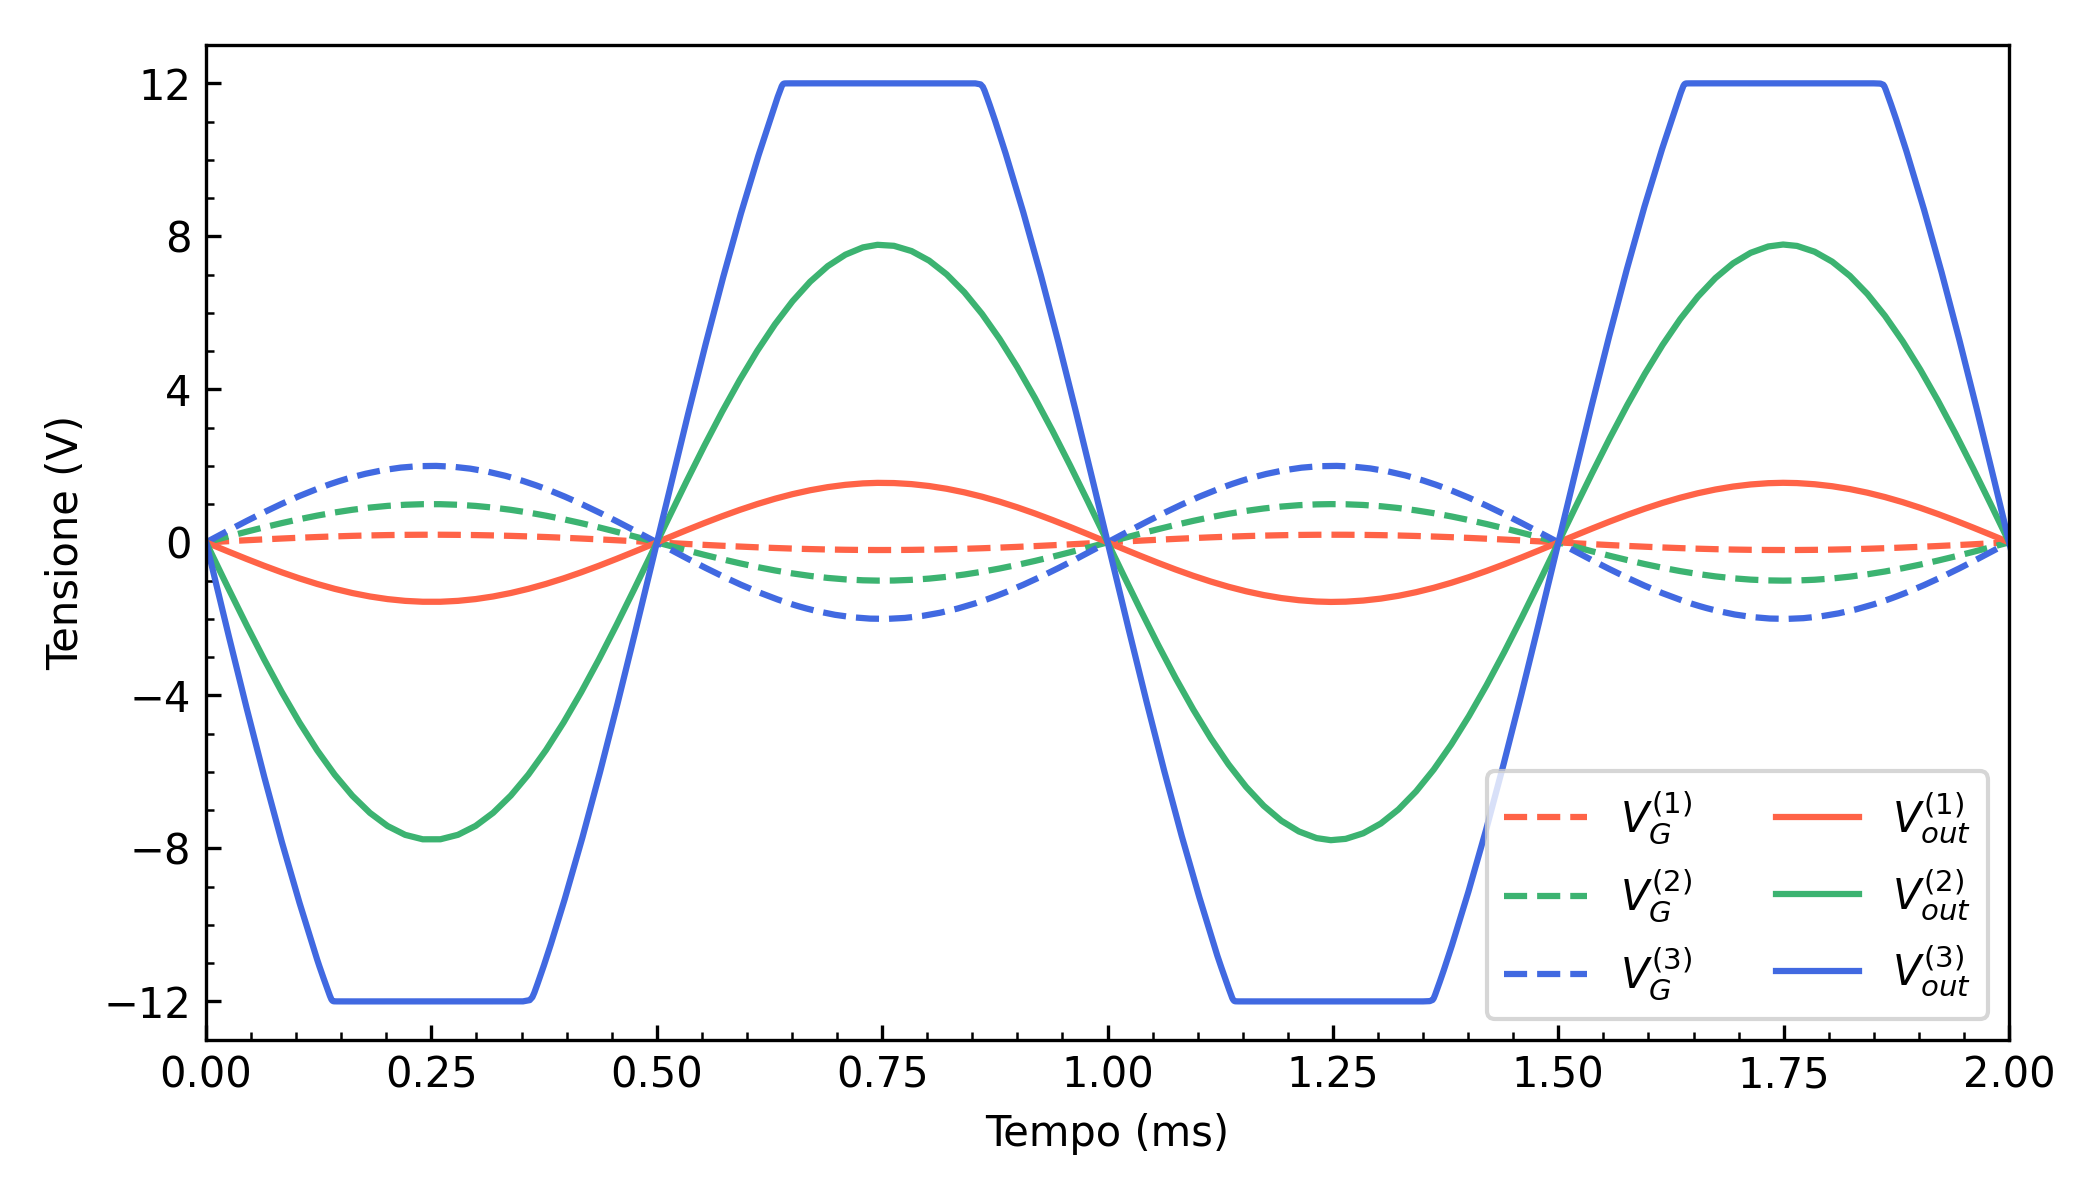
\includegraphics[width=0.5\textwidth]{images/lin_simulation}
\caption{\footnotesize Simulazione del circuito ottenuta con LTSpice XVII. Le linee
  tratteggiate rappresentano le tre tensioni di ingresso $V_{gen}^{(i)}$, mentre le linee continue rappresentano le corrispondenti tensioni di uscita $V_{out}^{(i)}$.}
\label{fig:lin_sim}
\end{wrapfigure}
%------------------------------------
un onda sinusoidale di $f_{gen}=1 \, \si{kHz}$, utilizzando il software LTSpice
XVII. In particolare, sono state effettuate tre simulazioni, corrispondenti a tre ampiezze diverse
del segnale del generatore:
%-----------------------------------
\begin{align*} V_{G}^{(1)} &= 0.2 \, \si{\volt}
  &
	V_{G}^{(2)}&=1 \, \si{\volt}
  &
	V_{G}^{(3)}&=2 \, \si{\volt}
\end{align*}
%-----------------------------------
I risultati delle simulazioni sono riportati in Figura \ref{fig:lin_sim} e risulta evidente come le prime due simulazioni confermino le considerazioni svolte
nella sezione precedente: il segnale di uscita risulta infatti invertito rispetto al segnale di
ingresso, e amplificato di un fattore di circa $8$.
La terza simulazione, invece, evidenzia il fenomeno di saturazione dell'amplificatore operazionale: esso, infatti, è alimentato da
una tensione continua di $\pm 12 \,\si{\volt}$ e per conservazione dell'energia questa sarà
la tensione massima che può fornire in output. Come mostrato nel grafico quindi, i massimi e
minimi del segnale in usicta risultano tagliati alla tensione di saturazione  $V_{s}=12 \, \si{\volt}$.
Dato il guadagno trovato in Equazione \ref{e:guadagno}, ci si aspetta che questo fenomeno si verifichi già ad una tensione di input $V_{G}\, \approx 1.5\, \si{\volt}$.

\subsection{Procedura di Acquisizione Dati }
Sfruttando i cursori di tipo tensione dell'oscilloscopio, vengono registrati separatamente
i massimi e i minimi del segnale di ingresso $V_{1}$ e del segnale di uscita $V_{out}$
aumentando progressivamente la tensione erogata dal generatore, partendo da un valore nominale
picco-picco di $V_{G}^{(pp)}=0.2 \, \si{\volt}$, fino a $V_{G}^{(pp)}=4 \, \si{\volt}$.

\subsection{Analisi dei dati}
In questa sezione ci si propone innanzitutto di verificare l'accordanza dei dati sperimentali
con le misure acquisite. Successivamente si cerca di ottenere una stima migliore
dell'amplificazione del circuito $G$. Per fare ciò si riportano in grafico le coppie $V_{in}$ e
$V_{out}$ e tramite un'interpolazione lineare si tenta di ricavare una nuova stima di $G$.
Inoltre, studiando la bontà del fit, si cerca di valutare la validità dell'ipotesi di linearità.

\subsubsection{Selezione dei dati}
In Figura \ref{fig:lin_sim} vengono riportate le misure di $V_{in}$ e $V_{out}$, a cui è stata
associata l'incertezza di lettura sommata quadraticamente all'incertezza di scala
%----------------------------------
\begin{align}\label{e:err_misure}
  \sigma_{V_{i}}= \sqrt{ \left(\sigma_{r} \times \si{\volt} / \text{div} \right)^{2} +
  \left( \sigma_{k} \times V_{i} \right)^{2}}
\end{align}
%----------------------------------
dove $\sigma_{k} = 1.7\%$ rappresenta l'errore di scala, mentre $\si{\volt}/ \text{div}$
corrisponde alla scala di acquisizione della misura. Come errore di lettura, si sceglie
di non utilizzare il valore fornito dal costruttore in quanto esso porterebbe ad
una sovrastima dell'errore. Si assume allora che il contributo maggiore all'errore di
lettura sia dato dalla discretizzazione che avviene durante la conversione analogico-digitale, per
cui l'errore massimo risulta $\Delta_{r}= 1 / 2^{n}$, dove $n$ rappresenta la risoluzione
dell'oscilloscopio. L'acquisizione delle misure è stata effettuata con $n=8 \text{ bit}$,
quindi, assumendo una distribuzione uniforme, si ha $\sigma_{r} = 0.002$.

%------------------------------------
\begin{figure}[h]
\centering
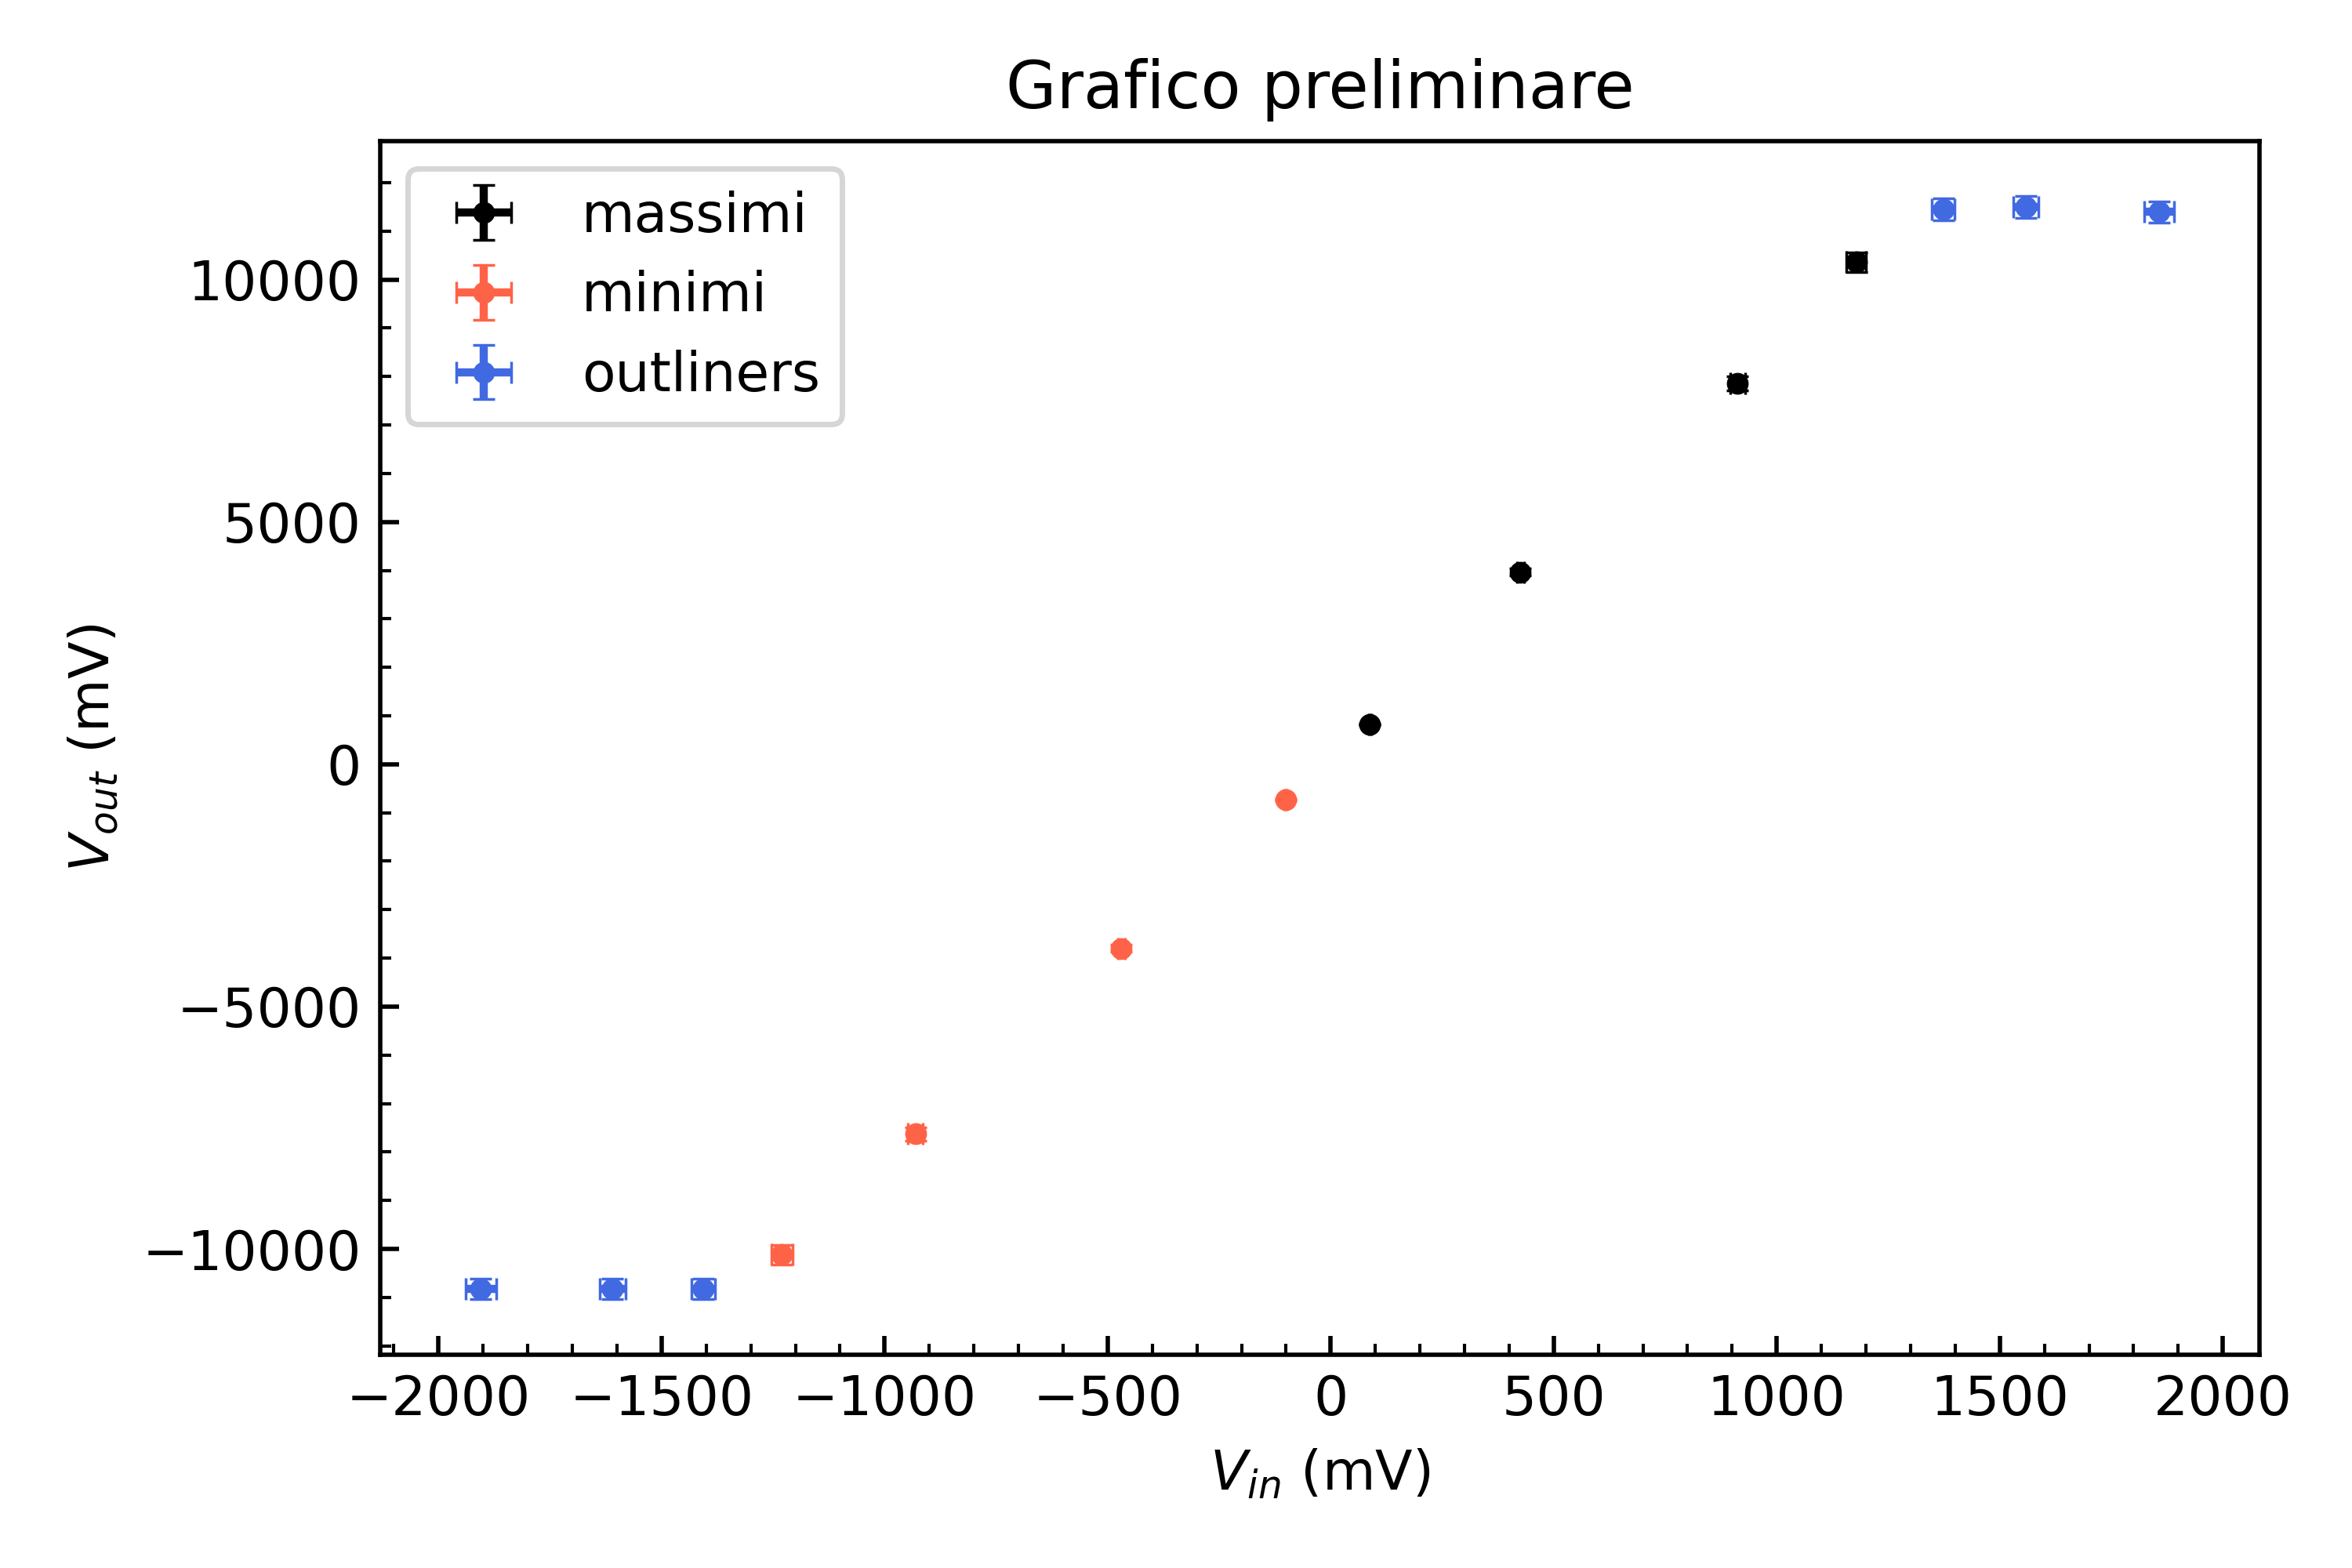
\includegraphics[width=0.7\textwidth]{images/grafico_esplorativo}
\caption{\footnotesize Grafico preliminare delle coppie $(V_{in},V_{out})$ dei massimi (in nero) e dei minimi (in rosso). Gli outliners dovuti al fenomeno di saturazione sono
evidenziati in blu.}\label{fig:lin_prelim}
\end{figure}
%------------------------------------
Dalla Figura \ref{fig:lin_sim} si può subito osservare come i valori di $V_{out}$ siano amplificati di un
fattore di circa $8$, come ci si aspettava. Si nota inoltre il fenomeno di saturazione
descritto nella Sezione \ref{s:sim}. Gli outliners corrispondenti non verranno considerati nelle
analisi successive.

\subsection{Interpolazione Lineare}
Si procede ora con la suddivisione dei dati in due set, corrispondenti ai massimi e ai minimi,
con l'obbiettivo di effettuare un interpolazione lineare su ciascun set e, dopo aver verificato
la compatibilità tra i parametri dei fit, fare una nuova interpolazione sui set unificati.
Non è infatti possibile stabilire a priori se l'amplificazione sia la stessa tra i due set
e se ci siano eventuali sfasamenti tra i due fit. Il coefficiente angolare dell'interpolazione
rappresenta una nuova stima dell'amplificazione $G$ e ci si aspetta che l'intercetta risulti
compatibile con lo zero.
Si noti però che gli errori associati alle ascisse ($V_{in}$) non risultano trascurabili rispetto a
quelli associati alle ordinate ($V_{out}$). Si decide allora di eseguire un primo fit senza considerare
l'errore sulle ascisse e di utilizzare il coefficiente angolare di questo fit per proiettare gli errori
di $V_{in}$ sulle ordinate, secondo la formula
%--------------------------------------
\begin{align}\label{e:proiezione}
 \sigma_{y} = \sqrt{ (m \times \sigma_{V_{in}})^{2} + \sigma_{V_{out}}^{2}}
\end{align}
%--------------------------------------
I risultati dei quattro fit sono riportati nella Tabella \ref{tab:fitmaxmin}. Si osservi però che il limitato numero
di misure di ciascun campione rende i fit poco significiativi e si attribuisce proprio a
questo problema la discrepanza tra gli errori a posteriori del fit dei massimi e quello dei
minimi: i primi infatti indicherebbero una leggera sottostima degli errori mentre i secondi
suggeriscono una forte sovrastima, che si rispecchia anche in un $\chi^{2}$ eccessivamente ridotto. I coefficienti angolari delle rette risultano inoltre scarsamente compatibili tra di loro ($\lambda = 2.2$). La compatibilità tra le due intercette risulta tuttavia ottima ($\lambda = 0.97$), ma la loro compatibilità con lo zero è discreta nel caso dei massimi ($\lambda = 1.83$), mentre nel caso dei minimi l'intercetta risulta addirittura incompatible
con lo zero ($\lambda = 3.21$).
\begin{table}[h]
\centering
\setlength{\tabcolsep}{10pt}
\begin{tabular}{ | c c | c c | c c | c c|  }
\hline
  \multicolumn{8}{|c|}{Parametri dei fit} \\
  \hline
  \multicolumn{4}{|c|}{Massimi} &
  \multicolumn{4}{c|}{Minimi} \\
  \hline
  \multicolumn{2}{|c}{$m_{\text{pre}}$} & \multicolumn{2}{c|}{$8.80 \pm 0.11$} &
  \multicolumn{2}{c}{$m_{\text{pre}}$} & \multicolumn{2}{c|}{$8.32 \pm 0.10$} \\
  $m_{\text{max}}$   &   $8.80 \pm 0.16$             &   $\sigma_{\text{p}}$              &   $ 202$   &   $m_{\text{min}}$   & $8.32 \pm 0.15 $            &  $\sigma_{\text p}$             & $10$ \\
  $q_{\text{max}}$   &   $ 64 \pm 35 \,\si{m\volt}$   &   $\chi^{2}/\text{ndf}$           &   $3.9/2$   &   $q_{\text{min}}$   & $110 \pm 35 \, \si{m\volt}$  & $\chi^{2} / \text{ndf}$        & $0.01/2$ \\
\hline
\end{tabular}
\caption{\footnotesize Si mostrano in tabella i coefficienti angolari dei fit preliminari
  $m_{\text{pre}}$ e i risultati dei fit con gli errori proiettati: in particolare si mostrano i
  coefficienti angolari $m_{i}$, le intercette $q_{i}$, gli errori a posteriori
  $\sigma_{\text{p}}$ e il chi quadro $\chi^{2}$ in relazione ai suoi gradi di libertà.}
\label{tab:fitmaxmin}
\end{table}

\noindent Si noti infine che nell'interpolazione sono stati considerati
sia i contributi degli errori di lettura che quelli di di guadagno verticale, in quanto
l'acquisizione delle misure è avvenuta a scale diverse. Questo tuttavia introduce una
correlazione tra le misure di cui il fit lineare non tiene conto e che quindi porta ad una
sottostima degli errori sui parametri e ad una compatibilità peggiore tra i due set.
Tuttavia, nonostante queste considerazioni, l'incompatibilità dell'intercetta dei minimi con
lo zero non può essere ignorata: essa infatti suggerisce un possibile errore sistematico di offset e vista la ottima compatibilità con l'intercetta del fit dei massimi si può assumere che
tale sistematica sia presente in entrambi i set e che sia costante, ovvero che si tratti di
una interferenza di fondo. Sebbene uno shift verticale costante non influenzi il coefficiente angolare dell'interpolazione (cioè la nuova stima di $G$) si sceglie comunque di non
unire i due campioni ma di analizzare le grandezze picco-picco delle tensioni in ingresso e in uscita,
secondo la formula $V_{pp}=V_{max} - V_{min}$. In questo modo infatti non solo si dovrebbe
riuscire a eliminare il contributo degli errori di shift verticale comuni a
entrambi i set, ma si possono ridurre anche eventuali sistematiche tra i due campioni, purchè
costanti per tutti i dati.\\

\noindent Come mostrato in precedenza, si procede prima con un fit
preliminare in cui si trascura il contributo degli errori delle ascisse per poi
sfruttare il coefficente angolare così ottenuto per proiettare gli errori sulle ordinate secondo l'Equazione \ref{e:proiezione}, potendo così fare un nuovo fit che tiene conto di
entrambe le incertezze. Nella Figura \ref{fig:lin_pp} sono riportati i risultati del fit.
%------------------------------------
\begin{figure}[h]
\centering
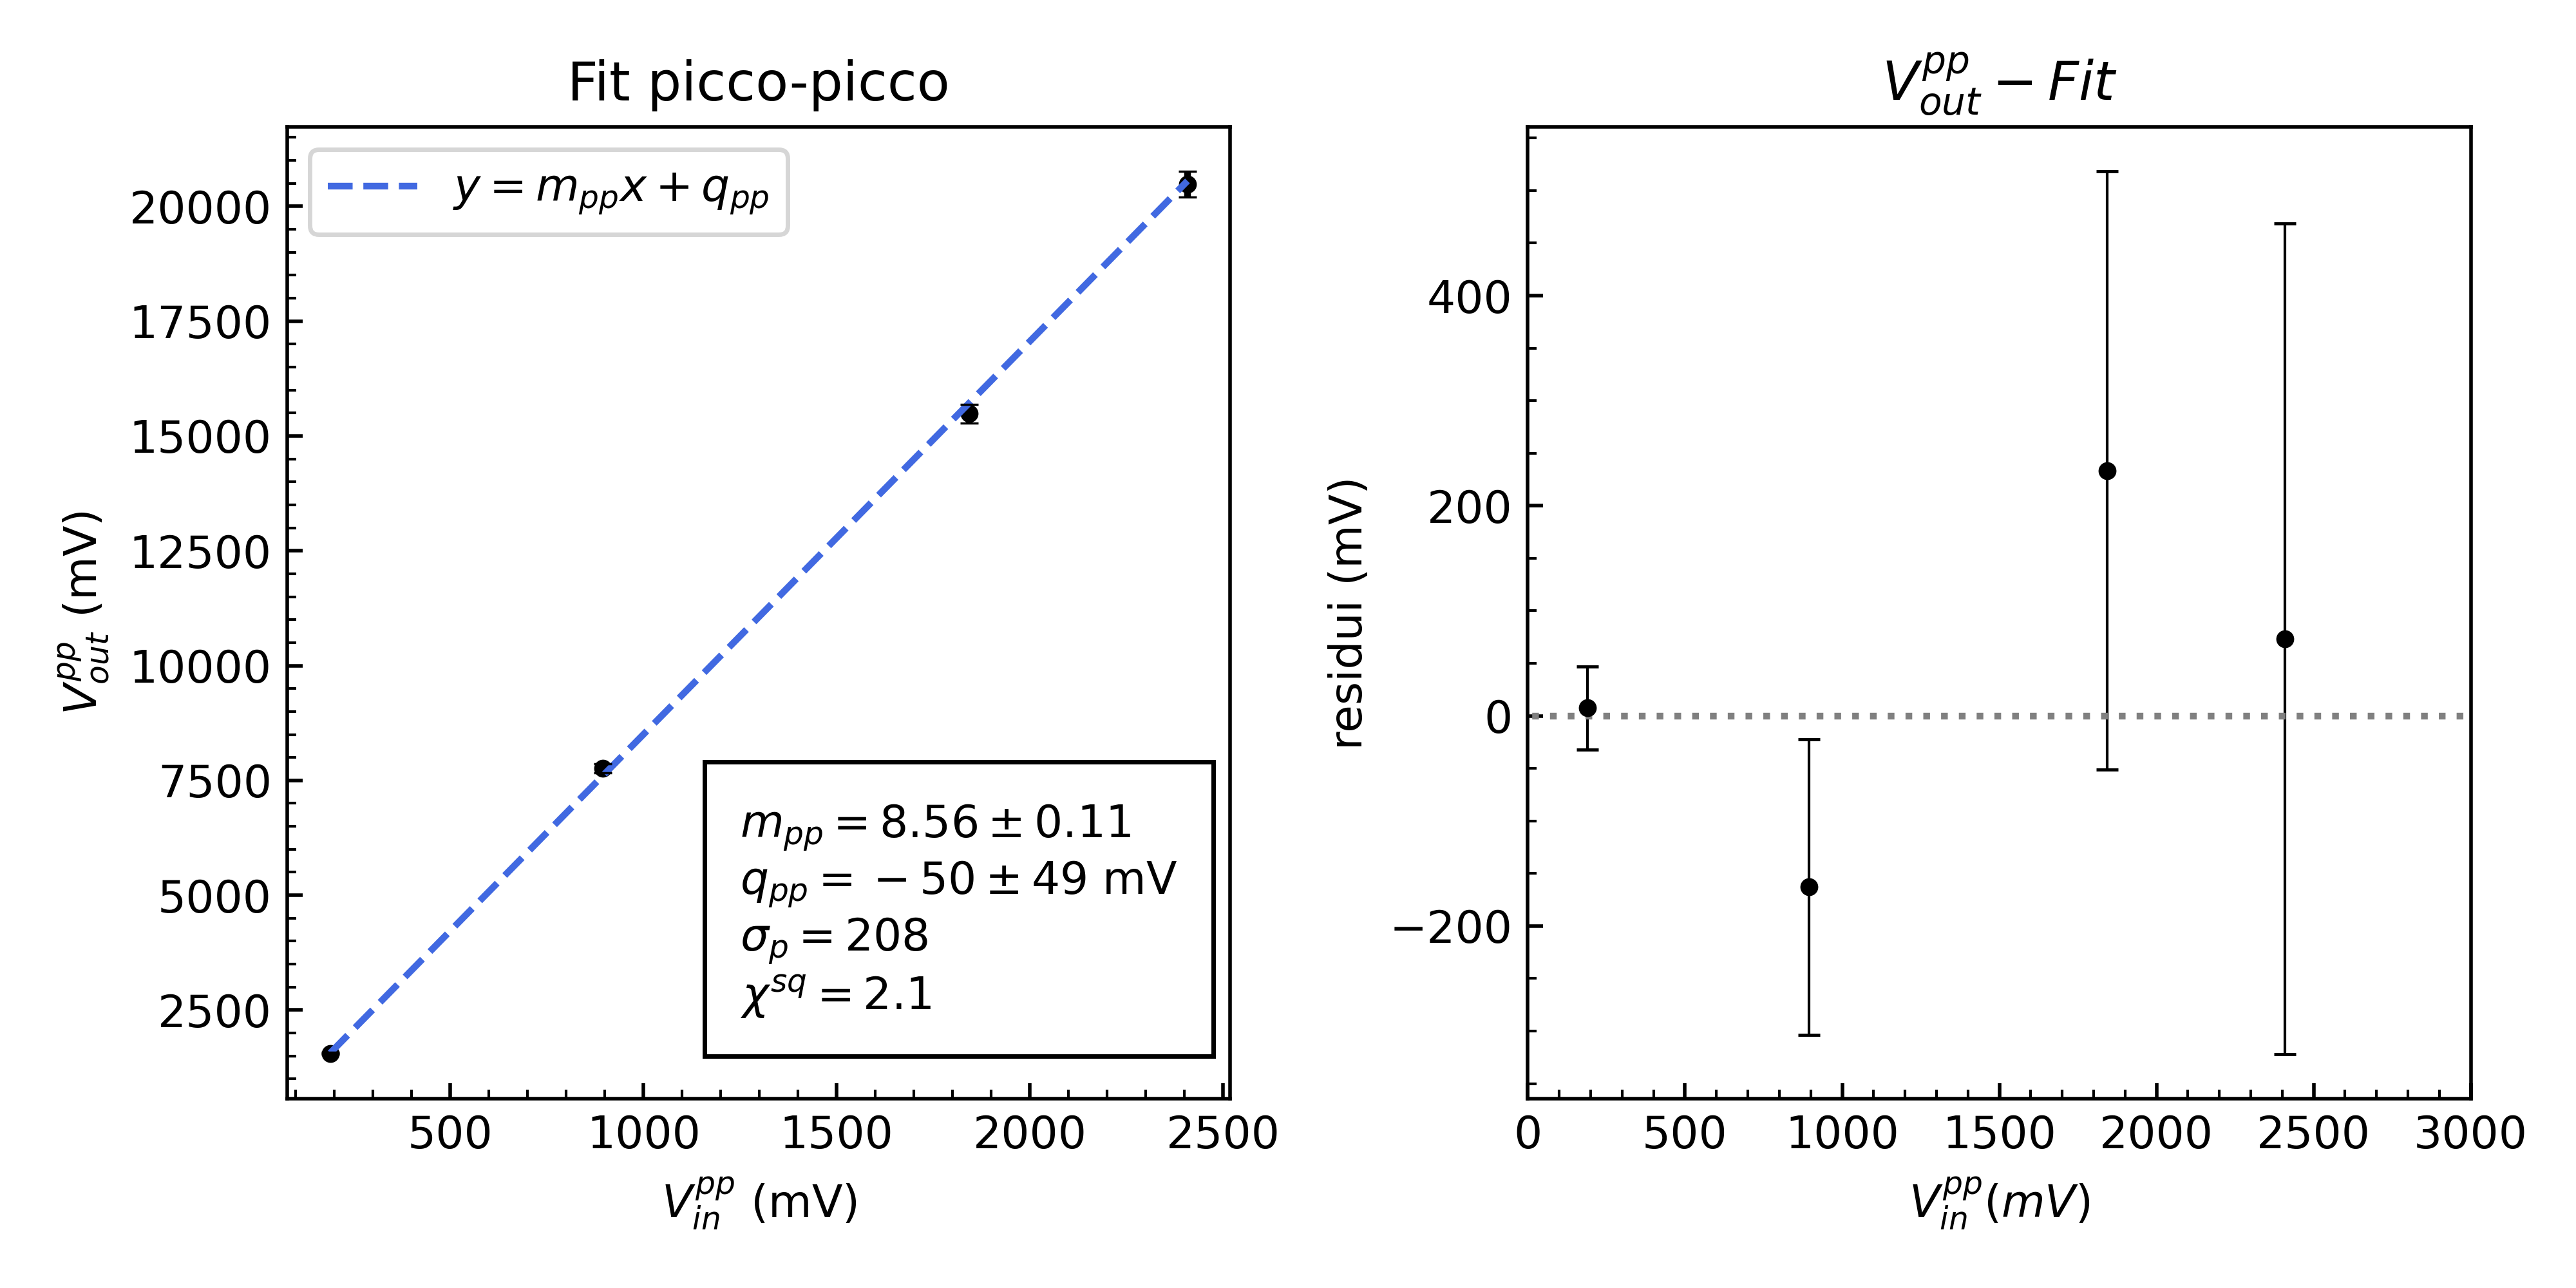
\includegraphics[width=0.9\textwidth]{images/grafico_pp}
\caption{\footnotesize Grafico}\label{fig:lin_pp}
\end{figure}
%------------------------------------
Si noti come la compatibilità dell'intercetta con lo zero sia ora $\lambda=1.0$, confermando quindi l'ipotesi di un offset verticale comune a entrambi i set che è stato rimosso una volta
presa la differenza. Anche il chi quadro risulta ora perfettamente compatibile con i suoi
gradi libertà ($\lambda=1.0$), confermando quindi l'ipotesi di andamento lineare dei
dati. Il coefficiente angolare, che rappresenta la nostra stima dell'amplificazione $G$,
risulta discretamente compatibile con il valore teorico previsto dall'Equazione
\ref{e:guadagno} ($\lambda = 1.5$).
Dal grafico dei residui si evidenzia inoltre una buona stima degli errori, con l'eccezione
dell'ultimo dato in cui l'incertezza è stata chiaramente sovrastimata.
Data la forte presenza di errori sistematici, si è scelto di non proseguire con l'analisi di
ulteriori indicatori indicatori statistici.

\subsubsection{Stime di G}
In Figura \ref{fig:all} sono state riportate tutte le stime dell'amplificazione $G$ del circuito calcolate nei paragrafi precedenti: dai coefficienti angolari dei fit dei massimi e dei
minimi sono state ottenute due stime $G_{\text{max}}$, $G_{\text{min}}$, compatibili tra di loro
($\lambda_{\text{max/min}}=2.2$), anche se debolmente. Da queste due stime si dicide di effettuare una media pesata, anchessa riportata in Figura \ref{fig:all}, ottenendo così un nuovo valore $<G>$ in ottimo accordo con la stima $G_{\text{pp}}$ ottenuta dall'analisi picco picco ($\lambda_{\text{pp/<>}}=0.1$). Queste ultime due stime presentano
inoltre una buona compatibilità con il valore $G_{\text{th}}$ previsto dall'Equazione \ref{e:guadagno}
$(\lambda_{\text{<>/th}} \approx \lambda_{\text{pp/th}} = 1.4)$.
Nonstante però tali compatibilità siano inferiori rispetto all'accordo che ha $G_{\text{min}}$ con l'aspettativa teorica ($\lambda_{\text{min/th}}=1.11$), si decide comunque di assumere come stima migliore dell'amplificazione
del circuito $G_{pp}$ in quanto si tratta del valore meno influenzato da errori sistematici, come spiegato nella Sezione \ref{s:lin_fit}.
%------------------------------------
\begin{figure}[h]
\centering
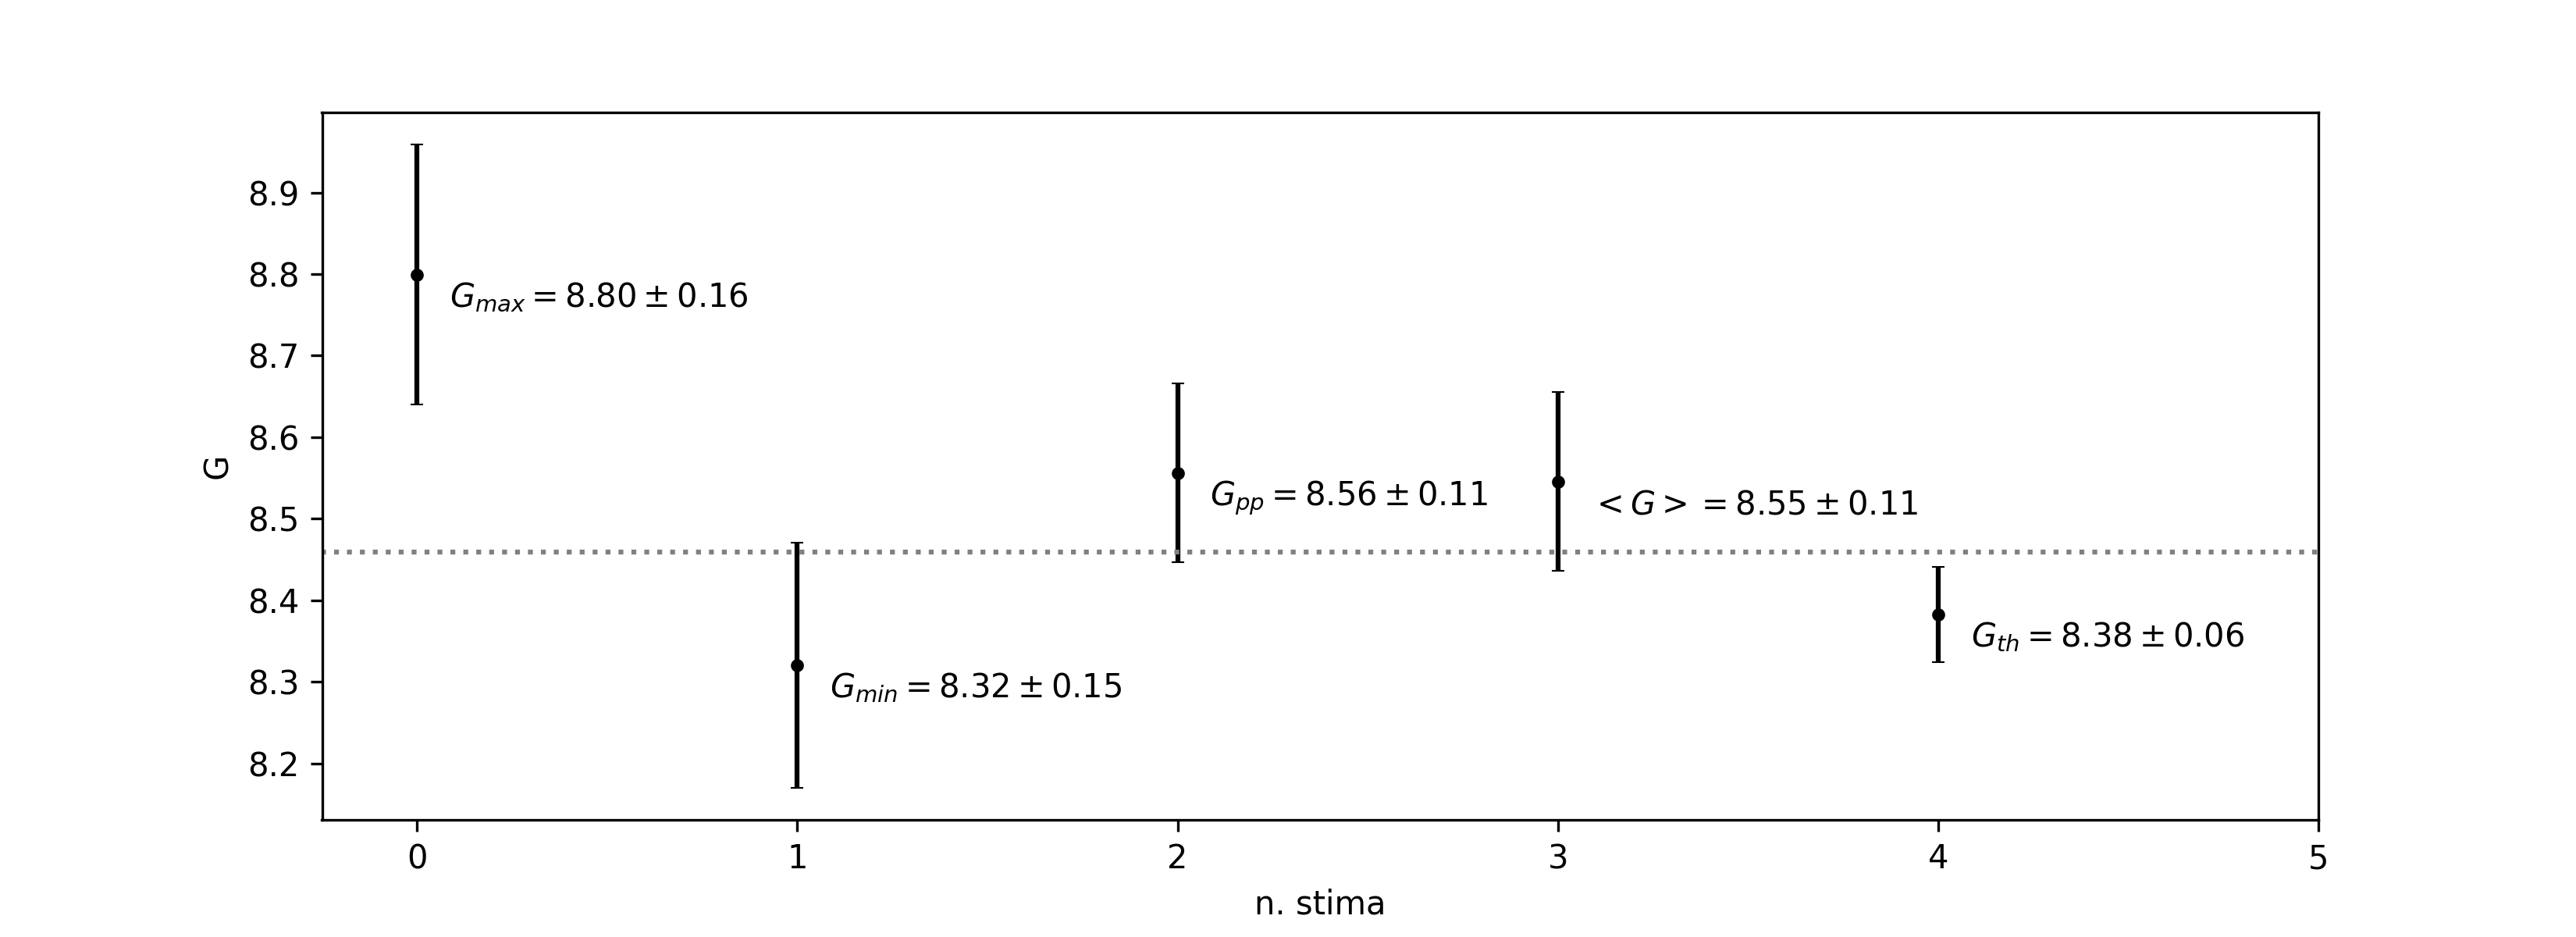
\includegraphics[width=1.1\textwidth]{images/grafico_all}
\caption{\footnotesize Grafico}\label{fig:all}
\end{figure}
%-------------------------------------
\end{document}
